\section{Green's functions}\label{sec:4.7}

The Bethe--Salpeter equation, which completes the hierarchy of \cref{sec:4.6}, needs quasiparticle energies and a screened interaction, and both are properties of one added electron. Put one extra electron into the conduction band of silicon. The other electrons move away from it and screen its charge, the lattice relaxes around it, and if it lies high enough in the band it can lose energy by creating an electron--hole pair or by emitting a phonon. The electron propagates dressed by its surroundings, with an energy that differs from its Kohn--Sham band energy and, in general, with a finite lifetime. The density response $R_{ee}$ of \cref{sec:4.1} does not follow this dressed electron, since the density operator moves an electron from one state to another and never changes their number. The function that does is the single-particle Green's function $\GF$: the amplitude that an electron added to the target at one time is still found in the same state at a later time. Its poles are the energies of the dressed electrons, the quasiparticles of the target, and the distance of each pole below the real axis is a decay rate. The treatment follows Refs.~\cite{bruus2004many}, \cite[Chaps.~3 and 7]{fetter1971quantum} and \cite[Chaps.~2 and 3]{mahan2000many}.

\subsection{The one-electron Green's function}

The Green's function changes the number of electrons, so we work in the grand-canonical state \cref{eq:2.5-grand}, with $\op{N}_e$ the electron number operator of \cref{sec:2.3}. Every Heisenberg operator in this section evolves with $H_\mu = H - \mu_{\mathrm{ch}}\op{N}_e$, so that $c(t) = \ee^{\ii H_\mu t}c\,\ee^{-\ii H_\mu t}$, and $E_i$ denotes an eigenvalue of $H_\mu$. Energies are then measured from the chemical potential: adding an electron to the $N$-electron state $|i\rangle$ to reach the $(N+1)$-electron state $|f\rangle$ costs $E_f - E_i$ in eigenvalues of $H_\mu$, which is the change of the total energy minus $\mu_{\mathrm{ch}}$. Let $c^\dagger_{\vect{k}}$ create an electron in a single-particle state labeled $\vect{k}$, with the spin and, in a crystal, the band index included in the label. The retarded Green's function is
\begin{equation}
  \GF^{\mathrm{R}}(\vect{k},t) = -\ii\,\Theta(t)\,\bigl\langle\{c_{\vect{k}}(t),\,c^\dagger_{\vect{k}}(0)\}\bigr\rangle ,
  \label{eq:4.7-GR}
\end{equation}
with the anticommutator $\{A, B\} = AB + BA$ and the average in the grand-canonical state. It has the form of the response function \cref{eq:4.1-kubo}, with an anticommutator in place of the commutator. The term $\langle c_{\vect{k}}(t)c^\dagger_{\vect{k}}\rangle$ is the overlap of the state with an electron added in $\vect{k}$ at time $0$ with the same state at time $t$: the amplitude that the added electron is still there. The term $\langle c^\dagger_{\vect{k}}c_{\vect{k}}(t)\rangle$ is the same amplitude for a hole, an electron removed from $\vect{k}$. The anticommutator makes $\GF^{\mathrm{R}}(\vect{k},0^+) = -\ii$ whatever the state, since $\{c_{\vect{k}}, c^\dagger_{\vect{k}}\} = 1$ (\cref{eq:2.3-anticomm}).

For independent electrons the amplitude is a pure phase. With $H_\mu = \sum_{\vect{k}}\xi_{\vect{k}}\,c^\dagger_{\vect{k}}c_{\vect{k}}$, where $\xi_{\vect{k}}$ is the energy of the orbital $\vect{k}$ of \cref{sec:2.3} measured from $\mu_{\mathrm{ch}}$, the Heisenberg operator is $c_{\vect{k}}(t) = c_{\vect{k}}\,\ee^{-\ii\xi_{\vect{k}}t}$ (\cref{sec:2.3}). The anticommutator in \cref{eq:4.7-GR} is then the number $\ee^{-\ii\xi_{\vect{k}}t}$, and with the transform of \cref{app:A.3} and $\omega \to \omega + \ii0^+$, as for every retarded function (\cref{sec:4.1}),
\begin{equation}
  \GF^{\mathrm{R}}_0(\vect{k},t) = -\ii\,\Theta(t)\,\ee^{-\ii\xi_{\vect{k}}t}, \qquad
  \GF^{\mathrm{R}}_0(\vect{k},\omega) = \frac{1}{\omega - \xi_{\vect{k}} + \ii0^+} .
  \label{eq:4.7-G0}
\end{equation}
The subscript $0$ marks the function without interactions. It has one pole, at the energy of the orbital, and it is independent of temperature and of which orbitals are occupied.

In an interacting target the same steps as in \cref{sec:4.1} lead to the eigenstates. Inserting a complete set of states between the operators, $\langle c_{\vect{k}}(t)c^\dagger_{\vect{k}}\rangle = \sum_{i,f}p_i\,|\langle f|c^\dagger_{\vect{k}}|i\rangle|^2\,\ee^{-\ii(E_f - E_i)t}$ and $\langle c^\dagger_{\vect{k}}c_{\vect{k}}(t)\rangle = \sum_{i,f}p_i\,|\langle f|c_{\vect{k}}|i\rangle|^2\,\ee^{+\ii(E_f - E_i)t}$, and the time integrals are those of \cref{eq:4.1-lehmann}. Since the two terms are added, not subtracted, both enter with a plus sign:
\begin{keyresult}[Lehmann representation of the Green's function]
\begin{equation}
  \begin{aligned}
  \GF^{\mathrm{R}}(\vect{k},\omega) &= \sum_{i,f}p_i\left[\frac{|\langle f|c^\dagger_{\vect{k}}|i\rangle|^2}{\omega - (E_f - E_i) + \ii0^+} + \frac{|\langle f|c_{\vect{k}}|i\rangle|^2}{\omega + (E_f - E_i) + \ii0^+}\right] \\
  &= \int\dd\omega'\,\frac{\SpecA(\vect{k},\omega')}{\omega - \omega' + \ii0^+} ,
  \end{aligned}
  \label{eq:4.7-lehmann}
\end{equation}
with the spectral function
\begin{equation}
  \begin{aligned}
  \SpecA(\vect{k},\omega) &= -\frac{1}{\pi}\Imag\GF^{\mathrm{R}}(\vect{k},\omega) \\
  &= \sum_{i,f}p_i\Bigl[|\langle f|c^\dagger_{\vect{k}}|i\rangle|^2\,\delta\bigl(\omega - (E_f - E_i)\bigr) + |\langle f|c_{\vect{k}}|i\rangle|^2\,\delta\bigl(\omega + (E_f - E_i)\bigr)\Bigr] .
  \end{aligned}
  \label{eq:4.7-A}
\end{equation}
The poles are at the energies needed to add an electron in $\vect{k}$, and at minus the energies released by removing one, each weighted by the probability that the added electron or hole is found in an exact eigenstate.
\end{keyresult}
This is the representation of Lehmann~\cite{lehmann1954uber}, and it shows that $\SpecA$ is positive, normalized, and tied to the occupations. It is positive since every weight in \cref{eq:4.7-A} is. Its integral over $\omega$ is $\sum_ip_i\langle i|c_{\vect{k}}c^\dagger_{\vect{k}} + c^\dagger_{\vect{k}}c_{\vect{k}}|i\rangle = 1$, which makes $\SpecA(\vect{k},\omega)$ a probability density in energy: the probability that an electron or hole put into $\vect{k}$ has the energy $\omega$. And the removal part alone counts the electrons already in $\vect{k}$. To see this, relabel $i \leftrightarrow f$ in the removal term; it becomes $\sum_{i,f}p_f\,|\langle f|c^\dagger_{\vect{k}}|i\rangle|^2\,\delta(\omega - (E_f - E_i))$, and on the energy shell $p_f = p_i\,\ee^{-\beta\omega}$, the detailed-balance step of \cref{eq:2.5-db}. The removal part is thus $\ee^{-\beta\omega}$ times the addition part, the two add up to $\SpecA$, and the removal part is $\SpecA\,\ee^{-\beta\omega}/(1 + \ee^{-\beta\omega}) = \SpecA\,n_{\mathrm{F}}(\omega)$. Its integral is $\langle c^\dagger_{\vect{k}}c_{\vect{k}}\rangle$:
\begin{equation}
  \langle c^\dagger_{\vect{k}}c_{\vect{k}}\rangle = \int\dd\omega\,\SpecA(\vect{k},\omega)\,n_{\mathrm{F}}(\omega) .
  \label{eq:4.7-occ}
\end{equation}
For independent electrons $\SpecA_0(\vect{k},\omega) = \delta(\omega - \xi_{\vect{k}})$ and \cref{eq:4.7-occ} is the Fermi function of \cref{eq:2.5-nF}. With interactions the occupation of a plane-wave state is no longer $n_{\mathrm{F}}(\xi_{\vect{k}})$, even at $T = 0$, because $\SpecA$ has weight at energies other than $\xi_{\vect{k}}$. Note that we normalize $\SpecA$ to one. Many texts, Refs.~\cite{bruus2004many,mahan2000many} among them, write $-2\Imag\GF^{\mathrm{R}}$ for the spectral function, which integrates to $2\pi$.

The spectral function is close to a measured quantity. In photoemission a photon removes an electron from the crystal, and the rate at a given energy and momentum of the outgoing electron is, in the simplest approximation, proportional to the removal part $\SpecA\,n_{\mathrm{F}}$; inverse photoemission measures the addition part. The analytic structure is that of \cref{sec:4.1}. By \cref{eq:4.7-lehmann}, $\GF^{\mathrm{R}}(\vect{k},z) = \int\dd\omega'\,\SpecA(\vect{k},\omega')/(z - \omega')$ is analytic in the upper half plane, and the advanced function $\GF^{\mathrm{A}}(\vect{k},\omega) = \GF^{\mathrm{R}}(\vect{k},\omega)^*$, nonzero only for $t < 0$, is its boundary value from below.

\subsection{The time-ordered function}

At $T = 0$ the perturbation theory of \cref{sec:4.8} produces a third function. The Dyson series \cref{eq:2.4-dyson} is a time-ordered exponential, and when it is used to expand a ground-state amplitude the operators come out in time order. The time-ordered Green's function is
\begin{equation}
  \GF(\vect{k},t) = -\ii\,\langle0|\mathrm{T}\,c_{\vect{k}}(t)\,c^\dagger_{\vect{k}}(0)|0\rangle
  = -\ii\,\Theta(t)\,\langle0|c_{\vect{k}}(t)\,c^\dagger_{\vect{k}}|0\rangle + \ii\,\Theta(-t)\,\langle0|c^\dagger_{\vect{k}}\,c_{\vect{k}}(t)|0\rangle ,
  \label{eq:4.7-GT}
\end{equation}
where $|0\rangle$ is the ground state of $H_\mu$ and the time-ordering symbol $\mathrm{T}$ puts the operator with the later time on the left, with a minus sign when two fermion operators are exchanged. For $t > 0$ it propagates an added electron forward in time, and for $t < 0$ a hole. The integral over $t > 0$ is that of the retarded function. The integral over $t < 0$ needs a factor $\ee^{+0^+t}$ to converge, $\ii\int_{-\infty}^0\dd t\,\ee^{\ii(\omega + E_f - E_0)t + 0^+t} = 1/(\omega + E_f - E_0 - \ii0^+)$, so
\begin{equation}
  \GF(\vect{k},\omega) = \sum_f\left[\frac{|\langle f|c^\dagger_{\vect{k}}|0\rangle|^2}{\omega - (E_f - E_0) + \ii0^+} + \frac{|\langle f|c_{\vect{k}}|0\rangle|^2}{\omega + (E_f - E_0) - \ii0^+}\right] .
  \label{eq:4.7-GTlehmann}
\end{equation}
The removal poles now lie above the real axis. At $T = 0$ every $E_f - E_0 \ge 0$, because $|0\rangle$ is the ground state of $H_\mu$ in all particle-number sectors. The addition poles therefore lie at $\omega > 0$ and the removal poles at $\omega < 0$. As a result, the time-ordered function equals $\GF^{\mathrm{R}}$ for $\omega > 0$ and $\GF^{\mathrm{A}}$ for $\omega < 0$, and both carry the same spectral function. In this section a $\GF$ without superscript and with a real time or frequency is the time-ordered function. With an imaginary argument it is the Matsubara function introduced below, and with a complex argument $z$ it is the function $\int\dd\omega'\,\SpecA(\vect{k},\omega')/(z - \omega')$, which unites them all.

\subsection{Self-energy and the Dyson equation}

How does an interaction change $\GF^{\mathrm{R}}$? Split $H_\mu = \sum_{\vect{k}}\xi_{\vect{k}}\,c^\dagger_{\vect{k}}c_{\vect{k}} + H_{\mathrm{int}}$, where $H_{\mathrm{int}}$ holds the Coulomb interaction between the electrons, their coupling to phonons, or any other term that is not a one-body energy. The Heisenberg operator obeys $\ii\,\partial_tc_{\vect{k}}(t) = [c_{\vect{k}}, H_\mu](t) = \xi_{\vect{k}}c_{\vect{k}}(t) + [c_{\vect{k}}, H_{\mathrm{int}}](t)$, by \cref{eq:2.3-bilinear}. Differentiating \cref{eq:4.7-GR}, the derivative of the step function gives $\delta(t)\langle\{c_{\vect{k}}, c^\dagger_{\vect{k}}\}\rangle = \delta(t)$, and
\begin{equation*}
  \ii\,\partial_t\GF^{\mathrm{R}}(\vect{k},t) = \delta(t) + \xi_{\vect{k}}\,\GF^{\mathrm{R}}(\vect{k},t) + \mathsf{F}^{\mathrm{R}}(\vect{k},t), \qquad
  \mathsf{F}^{\mathrm{R}}(\vect{k},t) = -\ii\,\Theta(t)\,\bigl\langle\{[c_{\vect{k}}, H_{\mathrm{int}}](t),\,c^\dagger_{\vect{k}}\}\bigr\rangle .
\end{equation*}
The function $\mathsf{F}^{\mathrm{R}}$ is a retarded correlation of the same kind, built from the operator $[c_{\vect{k}}, H_{\mathrm{int}}]$, which removes an electron from $\vect{k}$ and scatters the others. With $\ee^{\ii\omega t}$, the derivative $\ii\,\partial_t$ becomes $\omega$, and $(\omega - \xi_{\vect{k}})\,\GF^{\mathrm{R}} = 1 + \mathsf{F}^{\mathrm{R}}$. We define the self-energy $\Sigma^{\mathrm{R}}(\vect{k},\omega)$ as the ratio $\mathsf{F}^{\mathrm{R}}/\GF^{\mathrm{R}}$. This is possible because $\GF^{\mathrm{R}}(\vect{k},z)$ has no zeros in the upper half plane: there $\Imag\GF^{\mathrm{R}}(\vect{k},z) = -\Imag z\int\dd\omega'\,\SpecA(\vect{k},\omega')/|z - \omega'|^2 < 0$ by the positivity of $\SpecA$. Multiplying by $\GF^{\mathrm{R}}_0$ of \cref{eq:4.7-G0} gives the Dyson equation.
\begin{keyresult}[Dyson equation]
\begin{equation}
  \begin{gathered}
  \GF^{\mathrm{R}}(\vect{k},\omega) = \GF^{\mathrm{R}}_0(\vect{k},\omega) + \GF^{\mathrm{R}}_0(\vect{k},\omega)\,\Sigma^{\mathrm{R}}(\vect{k},\omega)\,\GF^{\mathrm{R}}(\vect{k},\omega), \\
  \GF^{\mathrm{R}}(\vect{k},\omega) = \frac{1}{\omega - \xi_{\vect{k}} - \Sigma^{\mathrm{R}}(\vect{k},\omega)} .
  \end{gathered}
  \label{eq:4.7-dyson}
\end{equation}
All the effects of the interaction on the propagation of one electron are in the self-energy $\Sigma^{\mathrm{R}}$, a complex function of energy.
\end{keyresult}
In a crystal, with $\vect{k}$ the crystal momentum and $n$ the band, the same steps make $\GF^{\mathrm{R}}$ and $\Sigma^{\mathrm{R}}$ matrices in the band indices, and \cref{eq:4.7-dyson} a matrix equation of the type \cref{eq:C.7-dyson}. In a translation-invariant target they are diagonal in $\vect{k}$, as we assume here.

So far \cref{eq:4.7-dyson} is a definition. Its content appears when it is iterated: $\GF^{\mathrm{R}} = \GF^{\mathrm{R}}_0 + \GF^{\mathrm{R}}_0\Sigma^{\mathrm{R}}\GF^{\mathrm{R}}_0 + \GF^{\mathrm{R}}_0\Sigma^{\mathrm{R}}\GF^{\mathrm{R}}_0\Sigma^{\mathrm{R}}\GF^{\mathrm{R}}_0 + \cdots$. The electron propagates freely, is scattered out of $\vect{k}$ and back by the interaction, propagates freely again, and so on, and $\Sigma^{\mathrm{R}}$ is the amplitude of one such excursion. \Cref{sec:4.8} computes $\Sigma$ with diagrams and shows that it is the sum of the excursions that cannot be cut into two by removing a single free propagator. A self-energy known only to low order then yields a Green's function to all orders, and no finite order of the series has the shifted, broadened pole that the closed form has (\cref{app:C.7}). This is what the width did for the intermediate state of \cref{sec:2.4}, where summing the repeated emission and reabsorption turned $\ii0^+$ into $\ii\varGamma_{\mathrm{w}}/2$ in \cref{eq:2.4-width}.

The sign of the width is fixed before any calculation. On the real axis, $\Sigma^{\mathrm{R}} = \omega - \xi_{\vect{k}} - 1/\GF^{\mathrm{R}}$ has the imaginary part $\Imag\GF^{\mathrm{R}}/|\GF^{\mathrm{R}}|^2$, so
\begin{equation}
  \Imag\Sigma^{\mathrm{R}}(\vect{k},\omega) = -\frac{\pi\,\SpecA(\vect{k},\omega)}{\bigl|\GF^{\mathrm{R}}(\vect{k},\omega)\bigr|^2} \le 0 .
  \label{eq:4.7-ImSigma}
\end{equation}
The large-frequency limit is fixed as well. At large $|\omega|$, the expansion $1/(\omega - \omega') = \omega^{-1} + \omega'\omega^{-2} + \cdots$ in \cref{eq:4.7-lehmann} gives $\GF^{\mathrm{R}} = \omega^{-1} + m_1\omega^{-2} + O(\omega^{-3})$, with $m_1 = \int\dd\omega\,\omega\,\SpecA = \langle\{[c_{\vect{k}}, H_\mu], c^\dagger_{\vect{k}}\}\rangle$ by the same steps as \cref{eq:4.1-tail}. Then $1/\GF^{\mathrm{R}} = \omega - m_1 + O(\omega^{-1})$, and $\Sigma^{\mathrm{R}}(\vect{k},\omega) \to m_1 - \xi_{\vect{k}} = \langle\{[c_{\vect{k}}, H_{\mathrm{int}}], c^\dagger_{\vect{k}}\}\rangle$. The self-energy tends to a static potential, linear in $H_{\mathrm{int}}$ and evaluated in the exact state. For the Coulomb interaction it is the mean-field (Hartree and exchange) potential, built with the exact occupations. Everything that depends on frequency, the retardation of the screening and the decay into other excitations, is in $\Sigma^{\mathrm{R}} - \Sigma^{\mathrm{R}}(\vect{k},\infty)$, which is analytic in the upper half plane and falls off at large $|\omega|$, and as a result obeys the Kramers--Kronig relations of \cref{app:C.5}.

\subsection{Quasiparticles}

Suppose the self-energy is small and varies slowly with $\omega$. The Green's function \cref{eq:4.7-dyson} is then large where its real denominator vanishes, at the quasiparticle energy $E_{\mathrm{qp}}(\vect{k})$ defined by
\begin{equation*}
  E_{\mathrm{qp}}(\vect{k}) - \xi_{\vect{k}} - \Real\Sigma^{\mathrm{R}}\bigl(\vect{k},E_{\mathrm{qp}}(\vect{k})\bigr) = 0 .
\end{equation*}
Near this energy we expand the real part to first order, $\omega - \xi_{\vect{k}} - \Real\Sigma^{\mathrm{R}} \simeq (\omega - E_{\mathrm{qp}})/z_{\mathrm{qp}}$, and keep the imaginary part at its value at $E_{\mathrm{qp}}$.
\begin{keyresult}[Quasiparticle]
\begin{equation}
  \begin{gathered}
  \GF^{\mathrm{R}}(\vect{k},\omega) \simeq \frac{z_{\mathrm{qp}}(\vect{k})}{\omega - E_{\mathrm{qp}}(\vect{k}) + \ii\varGamma_{\mathrm{qp}}(\vect{k})/2}, \\
  z_{\mathrm{qp}} = \Bigl[1 - \partial_\omega\Real\Sigma^{\mathrm{R}}(\vect{k},\omega)\big|_{E_{\mathrm{qp}}}\Bigr]^{-1}, \qquad
  \varGamma_{\mathrm{qp}} = -2z_{\mathrm{qp}}\Imag\Sigma^{\mathrm{R}}(\vect{k},E_{\mathrm{qp}}) .
  \end{gathered}
  \label{eq:4.7-qp}
\end{equation}
The real part of the self-energy shifts the energy, its slope sets the residue $z_{\mathrm{qp}}$, and its imaginary part sets the width $\varGamma_{\mathrm{qp}}$.
\end{keyresult}
In time, the pole at $E_{\mathrm{qp}} - \ii\varGamma_{\mathrm{qp}}/2$, in the lower half plane of the continued function, gives $\GF^{\mathrm{R}}(\vect{k},t) \simeq -\ii z_{\mathrm{qp}}\,\ee^{-\ii E_{\mathrm{qp}}t - \varGamma_{\mathrm{qp}}t/2}$: the added electron keeps the fraction $z_{\mathrm{qp}}$ of its amplitude in a state that oscillates at a definite energy and decays at the rate $\varGamma_{\mathrm{qp}}$. It is a resonance pole of the kind met in \cref{sec:4.1}, and $1/\varGamma_{\mathrm{qp}}$ is the quasiparticle lifetime. In the spectral function the pole is a Lorentzian of weight $z_{\mathrm{qp}}$ and full width $\varGamma_{\mathrm{qp}}$. In an interacting system $z_{\mathrm{qp}}$ is typically below one, and the rest of the sum rule, $1 - z_{\mathrm{qp}}$, is spread over a broad incoherent background: states in which the added electron has created electron--hole pairs, plasmons or phonons. Since the background is broad, its contribution to $\GF^{\mathrm{R}}(\vect{k},t)$ dephases within a time of order the inverse of its spread, and at later times the quasiparticle term is all that is left. The expansion requires $\varGamma_{\mathrm{qp}}$ to be small compared with the energy over which $\Sigma^{\mathrm{R}}$ changes, the condition of the Wigner--Weisskopf result of \cref{sec:2.4}. The quasiparticle is a useful concept only if it also lives long compared with its own period, $\varGamma_{\mathrm{qp}} \ll |E_{\mathrm{qp}}|$.

Whether that holds is a matter of phase space, and an estimate shows why quasiparticles are sharp near the Fermi level of a metal. An electron added in a state of energy $\xi_{\vect{k}} > 0$ above $\mu_{\mathrm{ch}}$ can decay by scattering off an electron of the Fermi sea, which leaves a hole below $\mu_{\mathrm{ch}}$ and two electrons above it. At $T = 0$ the Pauli principle forces all three energies into a window of width $\xi_{\vect{k}}$: the energy $\omega'$ lost by the added electron lies between $0$ and $\xi_{\vect{k}}$, and the partner must start between $-\omega'$ and $0$. The allowed region in these two energy variables is a triangle of area $\xi_{\vect{k}}^2/2$, so $\varGamma_{\mathrm{qp}} \propto \xi_{\vect{k}}^2$ and $\varGamma_{\mathrm{qp}}/\xi_{\vect{k}} \to 0$ as $\xi_{\vect{k}} \to 0$. Luttinger showed that $\Imag\Sigma^{\mathrm{R}}$ vanishes as $(\omega - \mu_{\mathrm{ch}})^2$ at every order of perturbation theory~\cite{luttinger1961analytic}. This is the basis of Landau's picture of a metal as a gas of weakly interacting quasiparticles. In a semiconductor the window is set by the gap instead. An electron at the bottom of the conduction band of silicon is in the lowest state with one extra electron, it has nothing to decay into, and its width is zero. Higher in the band, the electron--electron part of $\Imag\Sigma^{\mathrm{R}}$ stays zero until the electron has enough energy to create an electron--hole pair, at least $\Eg$ above the band edge. Below that energy the width comes from phonon emission alone, which \cref{sec:6.3} computes from the same \cref{eq:4.7-qp}.

The quasiparticle energies of silicon are material quantities, and the dark-matter rate needs them: the band edges set the threshold for electron excitation. They are computed by starting from the Kohn--Sham Hamiltonian in place of the free one. Its eigenvalues $\varepsilon_{n\vect{k}}$ already contain the exchange--correlation potential $v_{\mathrm{xc}}$, so $\Sigma - v_{\mathrm{xc}}$ takes the place of $\Sigma$ in the Dyson equation. With the approximation that the Kohn--Sham states diagonalize $\Sigma$, the quasiparticle condition expanded to first order about $\varepsilon_{n\vect{k}}$ gives
\begin{equation}
  E_{\mathrm{qp}}(n\vect{k}) \simeq \varepsilon_{n\vect{k}} + z_{\mathrm{qp}}\,\Real\bigl\langle\psi_{n\vect{k}}\big|\Sigma(\varepsilon_{n\vect{k}}) - v_{\mathrm{xc}}\big|\psi_{n\vect{k}}\bigr\rangle ,
  \label{eq:4.7-G0W0}
\end{equation}
the form in which first-principles quasiparticle corrections are evaluated~\cite{hybertsen1986electron}. A PBE calculation of silicon at its own lattice constant puts the indirect gap at \SI{0.602}{eV} (\cref{sec:3.4}), against the measured \SI{1.17}{eV} at low temperature~\cite[Eq.~(11)]{ramanathan2020ionization} (\SI{1.12}{eV} at \SI{300}{K}); the self-energy in the $GW$ approximation of \cref{sec:4.8} supplies most of the difference. \Cref{app:E.3} describes the calculation and its convergence.

\begin{workedexample}{A level coupled to a flat band}\label{we:4-level}
The simplest self-energy that can be computed exactly is that of a localized orbital $d$, of energy $E_{\mathrm{lev}}$, hybridized with a band of orbitals $\vect{k}$ of energies $\xi_{\vect{k}}$: an impurity level in a metal or an atomic orbital near a surface. The electrons do not interact with each other, and the model is Anderson's without his on-site repulsion~\cite{anderson1961localized}:
\begin{equation*}
  H_\mu = E_{\mathrm{lev}}\,d^\dagger d + \sum_{\vect{k}}\xi_{\vect{k}}\,c^\dagger_{\vect{k}}c_{\vect{k}} + \sum_{\vect{k}}\bigl(V_{\vect{k}}\,c^\dagger_{\vect{k}}d + V^*_{\vect{k}}\,d^\dagger c_{\vect{k}}\bigr) ,
\end{equation*}
with energies measured from $\mu_{\mathrm{ch}}$ and $d$, $d^\dagger$ the fermion operators of the level. The commutators $[d, H_\mu] = E_{\mathrm{lev}}d + \sum_{\vect{k}}V^*_{\vect{k}}c_{\vect{k}}$ and $[c_{\vect{k}}, H_\mu] = \xi_{\vect{k}}c_{\vect{k}} + V_{\vect{k}}d$ follow from \cref{eq:2.3-bilinear}. Let $\GF^{\mathrm{R}}_{dd}$ be defined by \cref{eq:4.7-GR} with $d$ for $c_{\vect{k}}$. Its equation of motion contains the mixed function $\GF^{\mathrm{R}}_{\vect{k}d}(t) = -\ii\Theta(t)\langle\{c_{\vect{k}}(t), d^\dagger\}\rangle$, whose own equation closes, since $\{c_{\vect{k}}, d^\dagger\} = 0$:
\begin{equation*}
  (\omega - E_{\mathrm{lev}})\,\GF^{\mathrm{R}}_{dd} = 1 + \sum_{\vect{k}}V^*_{\vect{k}}\,\GF^{\mathrm{R}}_{\vect{k}d}, \qquad
  (\omega - \xi_{\vect{k}})\,\GF^{\mathrm{R}}_{\vect{k}d} = V_{\vect{k}}\,\GF^{\mathrm{R}}_{dd} .
\end{equation*}
Eliminating $\GF^{\mathrm{R}}_{\vect{k}d}$ gives \cref{eq:4.7-dyson} with
\begin{equation}
  \Sigma^{\mathrm{R}}_d(\omega) = \sum_{\vect{k}}\frac{|V_{\vect{k}}|^2}{\omega - \xi_{\vect{k}} + \ii0^+} ,
  \label{eq:4.7-Sigmad}
\end{equation}
exact at every order in $V_{\vect{k}}$, and the same at every temperature and filling of the band: the anticommutators are numbers, and the averages never enter. The electron leaves $d$ for the band and returns, and \cref{eq:4.7-Sigmad} is the amplitude of one such excursion.

This is the level-shift function of the Wigner--Weisskopf problem, \cref{eq:D.3-resolvent}, at $z = \omega - E_{\mathrm{lev}} + \ii0^+$, with $|V_{\vect{k}}|^2$ in place of $|H'_{fi}|^2$. Take the flat band of \cref{we:2-continuum}: states spread uniformly over a width $E_{\mathrm{w}} = \SI{1}{eV}$ centered on $E_{\mathrm{lev}}$, all with the same $|V_{\vect{k}}|^2$, chosen so that the golden-rule rate $\varGamma = 2\pi|V_{\vect{k}}|^2\mathcal{D}_f$ is \SI{10}{meV}. \Cref{app:D.3} found $\Sigma^{\mathrm{R}}_d(E_{\mathrm{lev}}) = -\ii\varGamma/2$ with no shift, and a slope $\partial_\omega\Real\Sigma^{\mathrm{R}}_d = 2\varGamma/(\pi E_{\mathrm{w}}) = 0.0064$ at $E_{\mathrm{lev}}$. By \cref{eq:4.7-qp}, $E_{\mathrm{qp}} = E_{\mathrm{lev}}$, $z_{\mathrm{qp}} = 1/(1 - 0.0064) = 1.0064$ and $\varGamma_{\mathrm{qp}} = z_{\mathrm{qp}}\varGamma$. The spectral function is a Lorentzian of full width $\varGamma$ with peak height $2/(\pi\varGamma) = \SI{63.7}{eV^{-1}}$, and the exact $\SpecA_{dd}$ follows it to within 1.3 percent out to $10\varGamma$ from the peak (\cref{fig:4-level}). This is the Lorentzian line of \cref{eq:2.4-lorentz}, now as the energy distribution of an electron put into $d$, and its width is $-2\Imag\Sigma^{\mathrm{R}}_d$.

The residue exceeds one because the exact $\SpecA_{dd}$ vanishes outside the band, where $\Imag\Sigma^{\mathrm{R}}_d = 0$, while a Lorentzian of width $\varGamma$ puts the weight $2\varGamma/(\pi E_{\mathrm{w}}) = 0.0064$ beyond the band edges. The pole carries that weight back to the center, and the sum rule $\int\SpecA_{dd} = 1$ is satisfied by the exact function inside the band. The quasiparticle formulas also reproduce the corrections of \cref{app:D.3}: there the decay rate was $\varGamma$ divided by one minus the slope of the level-shift function, and the residue was the inverse of the same factor, which are $\varGamma_{\mathrm{qp}}$ and $z_{\mathrm{qp}}$. In the state with the band empty, $\GF^{\mathrm{R}}_{dd}(t) = -\ii\Theta(t)\langle0|d\,\ee^{-\ii H_\mu t}d^\dagger|0\rangle$ is $-\ii$ times the amplitude that an electron put into $d$ is still there, the $c_i(t)\,\ee^{-\ii E_{\mathrm{lev}}t}$ of \cref{eq:2.4-WW}, and $|\GF^{\mathrm{R}}_{dd}(t)|^2$ is the survival probability. The Green's function contains the Wigner--Weisskopf result, with the condition $\varGamma \ll E_{\mathrm{w}}$ appearing as the slow variation of $\Sigma^{\mathrm{R}}_d$. Temperature enters only the occupation: at $T = \SI{20}{meV}$ and $E_{\mathrm{lev}} = \SI{-30}{meV}$, \cref{eq:4.7-occ} gives $\langle d^\dagger d\rangle = 0.787$, against $n_{\mathrm{F}}(E_{\mathrm{lev}}) = 0.818$ for the isolated level.
\end{workedexample}

\begin{figure}[tbp]
  \centering
  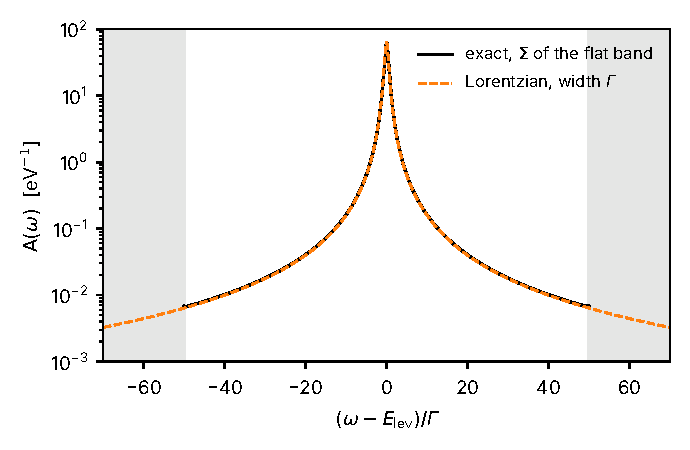
\includegraphics[width=0.68\linewidth]{figures/ch04/fig4_8b.pdf}
  \caption{Spectral function of a level of energy $E_{\mathrm{lev}}$ coupled to a flat band of width $E_{\mathrm{w}} = \SI{1}{eV}$ centered on $E_{\mathrm{lev}}$, with golden-rule rate $\varGamma = \SI{10}{meV}$ (the model of \cref{we:4-level}), on a logarithmic scale against $(\omega - E_{\mathrm{lev}})/\varGamma$. Solid: exact result, $\SpecA_{dd} = -\pi^{-1}\Imag[\omega - E_{\mathrm{lev}} - \Sigma^{\mathrm{R}}_d(\omega)]^{-1}$ with the self-energy of the band in the limit of a continuum, $\Sigma^{\mathrm{R}}_d = (\varGamma/2\pi)\ln[(\omega - E_{\mathrm{lev}} + E_{\mathrm{w}}/2)/(\omega - E_{\mathrm{lev}} - E_{\mathrm{w}}/2)]$ at $\omega + \ii0^+$. Dashed: Lorentzian of full width $\varGamma$ and unit weight. Shaded: outside the band, where the exact function vanishes (its two bound states lie exponentially close to the band edges and carry negligible weight) and the Lorentzian has the weight $2\varGamma/(\pi E_{\mathrm{w}}) = 0.0064$. Inside the band the exact function exceeds the Lorentzian by 1.0 percent at $|\omega - E_{\mathrm{lev}}| = \varGamma$ and by 1.3 percent at $10\varGamma$, because its quasiparticle residue is $1.0064$.}
  \label{fig:4-level}
\end{figure}

\subsection{Imaginary time}

At finite temperature two exponentials of the Hamiltonian appear in every average: $\ee^{-\ii H_\mu t}$ moves the operators in time, and $\ee^{-\beta H_\mu}$ weights the states. The second is the first at the imaginary time $t = -\ii\beta$. Matsubara used this to treat both on the same footing~\cite{matsubara1955new}. Define operators in imaginary time $\tau$ by
\begin{equation*}
  O(\tau) = \ee^{\tau H_\mu}\,O\,\ee^{-\tau H_\mu}, \qquad 0 \le \tau \le \beta ,
\end{equation*}
which is the Heisenberg operator $O(t)$ at $t = -\ii\tau$. Note that $c^\dagger(\tau)$ is not the adjoint of $c(\tau)$. The imaginary-time, or Matsubara, Green's function is
\begin{equation}
  \GF(\vect{k},\tau) = -\bigl\langle\mathrm{T}_\tau\,c_{\vect{k}}(\tau)\,c^\dagger_{\vect{k}}(0)\bigr\rangle ,
  \label{eq:4.7-Gtau}
\end{equation}
where $\mathrm{T}_\tau$ puts the operator with the larger $\tau$ on the left, with a minus sign for an exchange of fermion operators. Its use is that a perturbation expansion of $\ee^{-\beta H_\mu}$ and of $\ee^{\pm\tau H_\mu}$ in $H_{\mathrm{int}}$ is one Dyson series along the imaginary-time axis, with the same structure as \cref{eq:2.4-dyson}, and Wick's theorem then reduces every term to products of free Green's functions (\cref{sec:4.8}). The real-time time-ordered function of \cref{eq:4.7-GT}, however, has no expansion of this single-exponential form at $T > 0$ (\cref{app:D.11}), which is why the Matsubara function replaces it.

The cyclic property of the trace makes \cref{eq:4.7-Gtau} antiperiodic, $\GF(\vect{k},\tau - \beta) = -\GF(\vect{k},\tau)$ for $0 < \tau < \beta$ (\cref{app:D.10}). A function on $-\beta < \tau < \beta$ with this property is a Fourier series in the odd multiples of $\pi T$, the fermionic Matsubara frequencies $\omega^{\mathrm{F}}_j = (2j + 1)\pi T$ with integer $j$:
\begin{equation}
  \GF(\vect{k},\ii\omega^{\mathrm{F}}_j) = \int_0^\beta\dd\tau\,\ee^{\ii\omega^{\mathrm{F}}_j\tau}\,\GF(\vect{k},\tau), \qquad
  \GF(\vect{k},\tau) = T\sum_j\ee^{-\ii\omega^{\mathrm{F}}_j\tau}\,\GF(\vect{k},\ii\omega^{\mathrm{F}}_j) .
  \label{eq:4.7-Gmats}
\end{equation}
A correlation of two operators that each change the electron number by an even amount, such as two densities, is periodic instead, and its series runs over the bosonic frequencies $\omega^{\mathrm{B}}_j = 2j\pi T$. As $T \to 0$ both sets become dense on the imaginary axis.

The Lehmann form follows as before. For $0 < \tau < \beta$ only the ordering $c_{\vect{k}}(\tau)c^\dagger_{\vect{k}}$ appears, and inserting states leads to $\GF(\vect{k},\tau) = -\sum_{i,f}p_i|\langle f|c^\dagger_{\vect{k}}|i\rangle|^2\,\ee^{-(E_f - E_i)\tau}$. The integral in \cref{eq:4.7-Gmats} is elementary, and $\ee^{\ii\omega^{\mathrm{F}}_j\beta} = -1$:
\begin{equation*}
  \int_0^\beta\dd\tau\,\ee^{[\ii\omega^{\mathrm{F}}_j - (E_f - E_i)]\tau} = -\frac{1 + \ee^{-\beta(E_f - E_i)}}{\ii\omega^{\mathrm{F}}_j - (E_f - E_i)} .
\end{equation*}
Since $p_i\,\ee^{-\beta(E_f - E_i)} = p_f$, the weight becomes $(p_i + p_f)|\langle f|c^\dagger_{\vect{k}}|i\rangle|^2$, and the relabeling that led to \cref{eq:4.7-occ} shows that this is the weight of the spectral function at $\omega = E_f - E_i$.
\begin{keyresult}[Matsubara Green's function and analytic continuation]
\begin{equation}
  \GF(\vect{k},\ii\omega^{\mathrm{F}}_j) = \int\dd\omega'\,\frac{\SpecA(\vect{k},\omega')}{\ii\omega^{\mathrm{F}}_j - \omega'}, \qquad
  \GF^{\mathrm{R}}(\vect{k},\omega) = \GF(\vect{k},\ii\omega^{\mathrm{F}}_j \to \omega + \ii0^+) .
  \label{eq:4.7-continuation}
\end{equation}
The Matsubara and retarded functions are values of one analytic function, $\int\dd\omega'\,\SpecA(\vect{k},\omega')/(z - \omega')$, at the points $z = \ii\omega^{\mathrm{F}}_j$ and just above the real axis.
\end{keyresult}
In practice a Matsubara function computed in closed form is turned into the retarded one by the substitution $\ii\omega^{\mathrm{F}}_j \to \omega + \ii0^+$, made after every factor $\ee^{\ii\beta\omega^{\mathrm{F}}_j}$ has been replaced by $-1$. The continuation is unique, because the function falls off at large $|z|$ (\cref{app:C.5})~\cite{baym1961determination}. The Dyson equation carries over with the same self-energy evaluated at $z = \ii\omega^{\mathrm{F}}_j$, $\GF(\vect{k},\ii\omega^{\mathrm{F}}_j) = [\ii\omega^{\mathrm{F}}_j - \xi_{\vect{k}} - \Sigma(\vect{k},\ii\omega^{\mathrm{F}}_j)]^{-1}$, and for free electrons $\GF_0(\vect{k},\ii\omega^{\mathrm{F}}_j) = 1/(\ii\omega^{\mathrm{F}}_j - \xi_{\vect{k}})$.

Diagrams return their results as sums over Matsubara frequencies, and these are done by contour integration. The occupation is the simplest case. At $\tau = 0^-$ the time ordering puts $c^\dagger_{\vect{k}}$ on the left, $\GF(\vect{k},0^-) = \langle c^\dagger_{\vect{k}}c_{\vect{k}}\rangle$, and by \cref{eq:4.7-Gmats}
\begin{equation}
  \langle c^\dagger_{\vect{k}}c_{\vect{k}}\rangle = T\sum_j\ee^{\ii\omega^{\mathrm{F}}_j0^+}\,\GF(\vect{k},\ii\omega^{\mathrm{F}}_j) .
  \label{eq:4.7-occmats}
\end{equation}
The Fermi function $n_{\mathrm{F}}(z)$ has poles at the points $z = \ii\omega^{\mathrm{F}}_j$, each with residue $-T$, and the sum is a contour integral of $n_{\mathrm{F}}(z)\,\GF(\vect{k},z)$ around small circles that enclose them (\cref{fig:4-matsubara}a). Opened up, the circles become two lines that run along the real axis, above and below the cut of $\GF(\vect{k},z)$ (\cref{fig:4-matsubara}b). The jump of $\GF$ across the cut is $-2\pi\ii\SpecA$, by \cref{eq:4.7-lehmann}, and the sum becomes $\int\dd\omega\,\SpecA(\vect{k},\omega)\,n_{\mathrm{F}}(\omega)$, the occupation \cref{eq:4.7-occ}. \Cref{app:D.10} writes out the steps and the sum of two propagators that appears in every bubble diagram.

\begin{figure}[tbp]
  \centering
  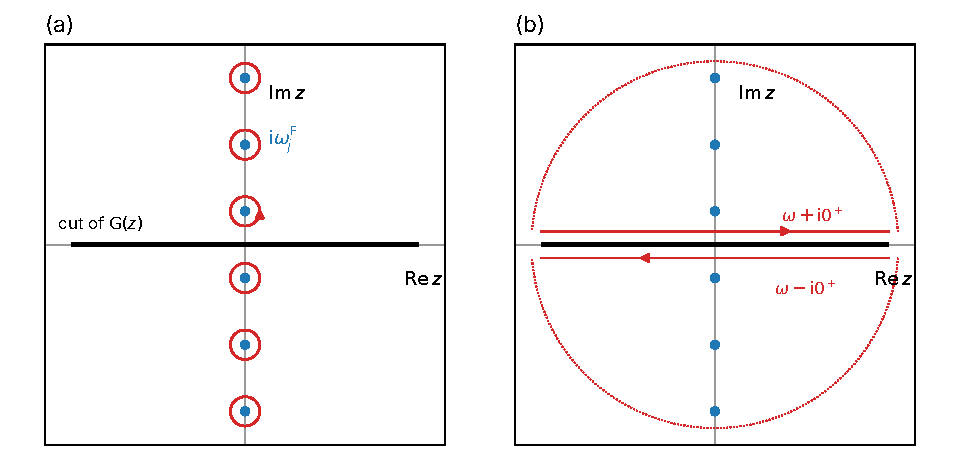
\includegraphics[width=\linewidth]{figures/ch04/fig4_8.pdf}
  \caption{Frequency sums by contour integration in the complex frequency plane $z$. (a) The fermionic Matsubara frequencies $\ii\omega^{\mathrm{F}}_j = (2j + 1)\pi\ii T$ (dots) are the poles of the Fermi function $n_{\mathrm{F}}(z)$, each with residue $-T$. A sum $T\sum_jg(\ii\omega^{\mathrm{F}}_j)$ is minus the integral of $n_{\mathrm{F}}(z)\,g(z)/2\pi\ii$ around small circles that enclose them counterclockwise. For $g = \GF(\vect{k},z)$ the only other singularity is the cut on the real axis (thick line), where the spectral function is nonzero. (b) The circles are merged into the boundaries of the upper and lower half planes: a line just above the real axis, at $\omega + \ii0^+$, run from left to right, and a line just below, at $\omega - \ii0^+$, run from right to left. The large arcs (dotted) contribute nothing when $n_{\mathrm{F}}(z)\,g(z)$ falls off faster than $1/|z|$ in every direction. The two lines see the retarded and advanced functions, and their difference, $-2\pi\ii\SpecA$, turns the sum into an integral over real frequencies.}
  \label{fig:4-matsubara}
\end{figure}

\subsection{The density response in imaginary time}

The density response obeys the same rules. For two operators $O_a$, $O_b$ that conserve the electron number, define
\begin{equation}
  R_{ab}(\vect{q},\tau) = -\frac{1}{\Vol}\bigl\langle\mathrm{T}_\tau\,O_a(\vect{q},\tau)^\dagger\,O_b(\vect{q},0)\bigr\rangle ,
  \label{eq:4.7-Rtau}
\end{equation}
with $O_a(\vect{q},\tau)^\dagger$ meaning $\ee^{\tau H_\mu}O_a(\vect{q})^\dagger\ee^{-\tau H_\mu}$ and no sign on exchange, since the operators are bosonic. The function is periodic in $\tau$ with period $\beta$, and its coefficients are taken at $\ii\omega^{\mathrm{B}}_j$. For $0 < \tau < \beta$ it is $-\Vol^{-1}\sum_{i,f}p_i\langle i|O_a^\dagger|f\rangle\langle f|O_b|i\rangle\,\ee^{-(E_f - E_i)\tau}$. Integrated with $\ee^{\ii\omega^{\mathrm{B}}_j\tau}$, now with $\ee^{\ii\omega^{\mathrm{B}}_j\beta} = +1$, each term gives $[\ee^{-\beta(E_f - E_i)} - 1]/[\ii\omega^{\mathrm{B}}_j - (E_f - E_i)]$ if the denominator is nonzero, and $\beta$ if it is zero, which happens only for $j = 0$ and $E_f = E_i$. With $p_i\,\ee^{-\beta(E_f - E_i)} = p_f$,
\begin{equation}
  R_{ab}(\vect{q},\ii\omega^{\mathrm{B}}_j) = \frac{1}{\Vol}\sum_{i,f}^{E_f \ne E_i}\frac{(p_i - p_f)\,\langle i|O_a^\dagger|f\rangle\langle f|O_b|i\rangle}{\ii\omega^{\mathrm{B}}_j - (E_f - E_i)}
  - \delta_{j0}\,\frac{\beta}{\Vol}\sum_{i,f}^{E_f = E_i}p_i\,\langle i|O_a^\dagger|f\rangle\langle f|O_b|i\rangle .
  \label{eq:4.7-Rmats}
\end{equation}
In the retarded Lehmann form \cref{eq:4.1-lehmann}, relabeling $i \leftrightarrow f$ in the antiresonant term turns its weight into $-p_f\langle i|O_a^\dagger|f\rangle\langle f|O_b|i\rangle$ and its denominator into $\omega - (E_f - E_i) + \ii0^+$, and the two terms combine into $(p_i - p_f)$ times one pole. That is the sum in \cref{eq:4.7-Rmats} with $\ii\omega^{\mathrm{B}}_j \to \omega + \ii0^+$.
\begin{keyresult}[Response function from imaginary time]
\begin{equation}
  R_{ab}(\vect{q},\omega) = R_{ab}(\vect{q},\ii\omega^{\mathrm{B}}_j \to \omega + \ii0^+), \qquad j > 0 .
  \label{eq:4.7-Rcont}
\end{equation}
The retarded response function of \cref{sec:4.1} is the analytic continuation of the imaginary-time correlation function \cref{eq:4.7-Rtau} from the positive bosonic Matsubara frequencies.
\end{keyresult}
The term with $\delta_{j0}$ is not part of the continuation, which uses the points $j > 0$ alone, and it has a physical meaning. It comes from matrix elements between states of equal energy, and it is the extra term proportional to $\beta$ that distinguishes the isothermal static response from the limit $\omega \to 0$ of $R_{ab}(\vect{q},\omega)$, the isolated response of \cref{sec:4.1}~\cite{kubo1957statistical}. The value at $\omega^{\mathrm{B}}_0 = 0$ is the isothermal one, since it is a derivative of an equilibrium average in which the field has been present long enough for the target to stay in equilibrium with the bath.

For independent electrons the imaginary-time route writes the response as a sum over one fermionic frequency of a product of two free Green's functions. With $O_a = O_b = n_e(\vect{q})$ from \cref{eq:2.3-nq} and occupations $n_{\mathrm{F}}(\xi_{\vect{k}})$, \cref{app:D.10} evaluates \cref{eq:4.7-Rtau} directly and shows that it equals
\begin{equation}
  R^0(\vect{q},\ii\omega^{\mathrm{B}}_j) = \frac{1}{\Vol}\sum_{\vect{k}}T\sum_{j'}\GF_0(\vect{k},\ii\omega^{\mathrm{F}}_{j'})\,\GF_0(\vect{k} + \vect{q},\ii\omega^{\mathrm{F}}_{j'} + \ii\omega^{\mathrm{B}}_j)
  = \frac{1}{\Vol}\sum_{\vect{k}}\frac{n_{\mathrm{F}}(\xi_{\vect{k}}) - n_{\mathrm{F}}(\xi_{\vect{k}+\vect{q}})}{\ii\omega^{\mathrm{B}}_j + \xi_{\vect{k}} - \xi_{\vect{k}+\vect{q}}} ,
  \label{eq:4.7-bubble}
\end{equation}
with the sum over $\vect{k}$ including spin. Continued to $\omega + \ii0^+$, it is the independent-electron response whose imaginary part is the transition sum \cref{eq:2.5-indep}, and \cref{sec:4.5} evaluates it for the electron gas. The product of two propagators, one carrying the electron from $\vect{k}$ to $\vect{k} + \vect{q}$ and one carrying the hole back, is the bubble diagram of \cref{sec:4.8}. With interactions the same continuation holds term by term, and the diagrams of the next section compute $\Sigma$ and $R$ as Matsubara sums, which \cref{eq:4.7-continuation,eq:4.7-Rcont} then carry to the real frequencies at which a dark-matter particle deposits its energy.
